\documentclass[../opis-rozwiazania.tex]{subfiles}

\begin{document}
\label{communication-sec}

\subsection{Utworzenie sesji}

Celem tej sekwencji komunikacji jest odnalezienie istniejącej już sesji lub stworzenie nowej.
Zakładamy, że w systemie istnieje wolna maszyna.
W przeciwnym przypadku zgłaszamy użytkownikowi błąd. Proces przedstawiony jest na rysunku \ref{figure:diagrams:sequence_diagrams:tworzenie_sesji}.

\begin{figure}[ht!]
  \centering
  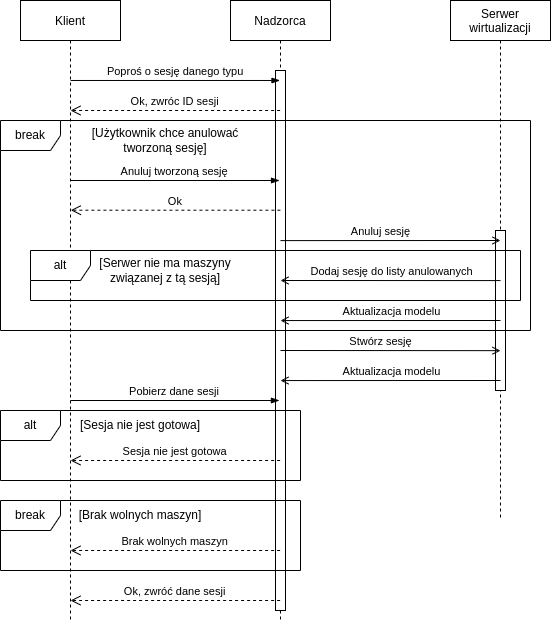
\includegraphics[width=0.8\textwidth]{../diagrams/sequence_diagrams/tworzenie_sesji.png}
  \caption{Sekwencja komunikacji utworzenia sesji}
  \label{figure:diagrams:sequence_diagrams:tworzenie_sesji}
\end{figure}

Po prośbie użytkownika nadzorca znajduje wolną maszynę i prosi odpowiadający serwer wirtualizacji, aby spróbował utworzyć z nią sesję dla użytkownika.
W przypadku sukcesu serwer wysyła informację o zmianie modelu.
W przeciwnym przypadku nadzorca powtarza wyszukanie wolnej maszyny.
Stan otrzymanej maszyny decyduje, czy nadzorca musi powtórzyć wyszukiwanie (m.in. czy sesja do niej przypisana należy do tego użytkownika).

Może się zdarzyć, że użytkownik anuluje wyszukiwanie.
Jeżeli maszyna jest już przydzielona, to serwer wirtualizacji jest powiadamiany o anulowaniu sesji.
Jeżeli nie została jeszcze utworzona, to nadzorca przerywa wyszukiwanie lub wyłącza ją.

\subsection{Zakończenie sesji}

Sekwencja ta zainicjowana jest poprzez utracenie połączenia z użytkownikiem maszyny.
Serwer powiadamia o tym fakcie nadzorców, po czym oczekuje na polecenie wyłączenia maszyny przesłane przez nadzorcę. Serwer może odmówić z powodu różnic modelu, lub jeżeli maszyna znów jest używana przez użytkownika, ignorując wiadomość. Proces przedstawiony jest na rysunku \ref{figure:diagrams:sequence_diagrams:konczenie_sesji}.

\begin{figure}[ht!]
  \centering
  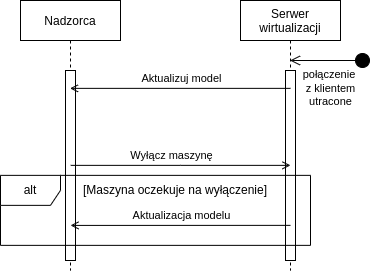
\includegraphics[width=0.6\textwidth]{../diagrams/sequence_diagrams/konczenie_sesji.png}
  \caption{Sekwencja komunikacji zakończenia sesji}
  \label{figure:diagrams:sequence_diagrams:konczenie_sesji}
\end{figure}

\subsection{Aktualizacja stanu}

Rysunek \ref{figure:diagrams:sequence_diagrams:konczenie_sesji} przedstawia sekwencję aktualizacji modelu. Nadzorca może w każdej chwili poprosić wszystkie serwery wirtualizacji
o przesłanie ich aktualnego stanu poprzez wspólną kolejkę do serwerów wirtualizacji (rozdział \ref{modules:broker}, kolejka \ref{modules:broker:queue-virtsrv}).
Serwery muszą bezwarunkowo odpowiedzieć aktualnym stanem do wspólnej kolejki zwrotnej (rozdział \ref{modules:broker}, kolejka \ref{modules:broker:queue-overseers}).

\begin{figure}[ht!]
  \centering
  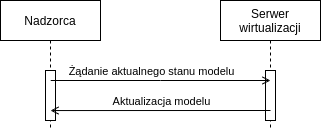
\includegraphics[width=0.6\textwidth]{../diagrams/sequence_diagrams/aktualizacja_stanu.png}
  \caption{Sekwencja komunikacji aktualizacji stanu systemu}
  \label{figure:diagrams:sequence_diagrams:aktualizacja_stanu}
\end{figure}

\subsection{Włączenie maszyny}

Nadzorca może poprosić konkretny serwer wirtualizacji, aby utworzył maszynę o wybranej nazwie.
Jeżeli maszyna nie istnieje, to zostanie uruchomiona, a serwer odeśle powiadomienie o zmianie modelu zbiorczą kolejką (rozdział \ref{modules:broker}, kolejka \ref{modules:broker:queue-overseers}).
W przeciwnym wypadku nie zrobi nic.

\begin{figure}[ht!]
  \centering
  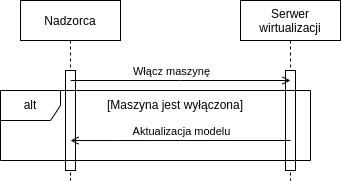
\includegraphics[width=0.6\textwidth]{../diagrams/sequence_diagrams/wlaczenie_maszyny.png}
  \caption{Sekwencja komunikacji włączenia maszyny}
  \label{figure:diagrams:sequence_diagrams:wlaczenie_maszyny}
\end{figure}

\subsection{Wyłączenie maszyny}

Nadzorca może poprosić konkretny serwer wirtualizacji, aby wyłączył konkretną maszynę wirtualną.
Jeżeli maszynę można wyłączyć, to zostanie ona wyłączona.
Następnie serwer wirtualizacji odeśle powiadomienie o zmianie modelu zbiorczą kolejką (rozdział \ref{modules:broker}, kolejka \ref{modules:broker:queue-overseers}).
W przeciwnym wypadku nie zrobi nic.

\begin{figure}[ht!]
  \centering
  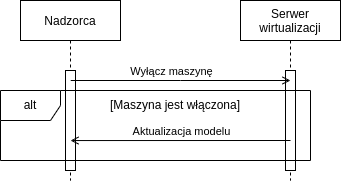
\includegraphics[width=0.6\textwidth]{../diagrams/sequence_diagrams/wylaczenie_maszyny.png}
  \caption{Sekwencja komunikacji wyłączenia maszyny}
  \label{figure:diagrams:sequence_diagrams:wylaczenie_maszyny}
\end{figure}

\end{document}